\documentclass{article}

\usepackage[ngerman]{babel}
\usepackage[utf8]{inputenc}
\usepackage[T1]{fontenc}
\usepackage{hyperref}
\usepackage{csquotes}
\usepackage[a4paper]{geometry}
\usepackage{graphicx}
\usepackage{float}
\usepackage{caption}

\usepackage[
    backend=biber,
    style=apa,
    sortlocale=de_DE,
    natbib=true,
    url=false,
    doi=false,
    sortcites=true,
    sorting=nyt,
    isbn=false,
    hyperref=true,
    backref=false,
    giveninits=false,
    eprint=false]{biblatex}
\addbibresource{../references/bibliography.bib}


\title{Diskriminierung durch KI}
\author{Luisa Rudin}
\date{\today}



\begin{document}

\maketitle

\begin{figure}[ht]
    \centering
    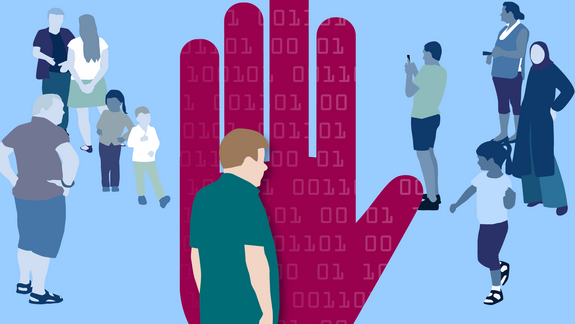
\includegraphics[width=1\textwidth]{KI Diskriminierung.jpg}
    \caption{}
    \label{fig:Diskriminierung}
\end{figure}

\section{Fragestellung}
    \textbf{\textit{
    Wie kann die Diskriminierung durch KI-Algorithmen verhindert werden und welche ethischen Massnahmen sind notwendig?}}


\tableofcontents

\section{\textit{Einleitung}}
Künstliche Intelligenz, auch abgekürzt als 'KI', ist ein von Menschegemachtes Computerprogramm.. Es handelt sich um eine Technologie, die unser Leben stark beeinflusst hat und in den vergangenen Jahren enorm mächtig geworden ist. KI-Systeme werden durch komplexe Algorithmen trainiert, die von Personen entwickelt werden. Diese Algorithmen dienen als Schritt-für-Schritt-Anleitung, um bestimmte Aufgaben zu lösen, die menschliche Intelligenz verlangen.  Um eine KI zu trainieren, werden als Erstes Daten gesammelt. Dann wird ein Modell ausgesucht, dass der KI anweisungen gibt, was sie lernen soll. Anschliessend "füttert" man die KI mit den gesammelten Daten und anhand dessen lernt sie Zusammenhänge und Muster. Dies geschieht durch wiederholtes Testen und Anpassen der internen Parameter des Modells, bis die Vorhersagen oder Entscheidungen der KI so genau wie möglich sind. Je nach Art der Daten und der gewünschten Aufgaben können verschiedene Lernmethoden zum Einsatz kommen. Beim überwachten Lernen wird die KI mit Beispielen trainiert, bei denen die richtige Antwort bekannt ist. Beim unüberwachten Lernen versucht die KI, Muster in den Daten selbstständig zu finden. Beim bestärkenden Lernen lernt die KI durch Belohnungen und Bestrafungen, ähnlich wie ein Kind, das durch positives Feedback lernt.

\section{\textit{Wie ensteht die Diskriminierung?}}
Die Diskriminierung beginnt in den Daten, die gesammelt werden um die KI zu trainieren. Den aus denen lernt der algorithmus, das eine bestimmte Personengruppe ein wiederholendes Muster in der Geschichte hat. Somit lernt die KI auch vorurteile, die von Menschen veröffentlicht wurden. Zum BEispiel: Eine KI lernt von einem Dokument, dass dunkelhäutige in der früheren Zeit benachteiligt wurden und deshalb oft kriminell waren. Also lernt die KI grob gesagt: Dunkelhäutige MEnschen sind krminell." Diese KI kann zum Beispiel für das aussortieren von Bewerbern in einem Konzern verantwortlich sein. Das führt dazu, dass er alle dunkelhäutigen Bewerber aussortiert und sie somit diskriminiert aufgrund der Daten von der sie gelernt hat. So ein ähnliches Beispiel ist tatsächlich passiert. Dazu steht unter "Beispiel Amazon" mehr. Solche diskriminierungsfälle sind shr problematisch, da immer mehr von KI gestuert wird und sie auch Entscheidungen treffen können und so viele Personen, wenn auch ohne Absicht der hersteller der KI, benachteiligt werden. 

\begin{figure}[ht]
    \centering
    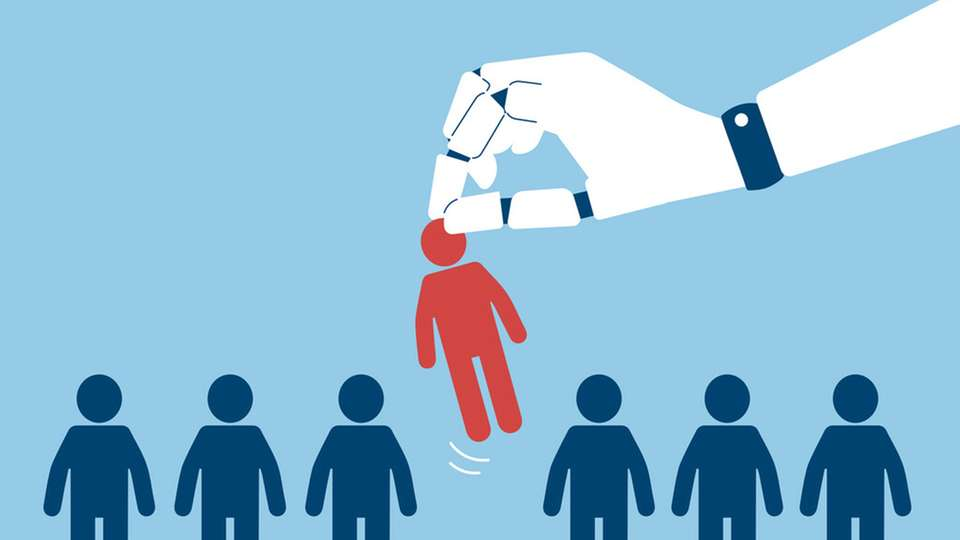
\includegraphics[width=0.5\textwidth]{KI Diskriminierung 2.jpg}
    \caption{}
    \label{fig:Diskriminierung}
\end{figure}

\section{\textit{Auswirkungen der Diskriminierung}}
Auf gesellschaftlicher Ebene kann KI die bestehenden sozialen Ungleichheiten verschärfen. Wenn zum Beispiel eine KI bei der Auswahl von Bewerbern für Jobs bestimmte Gruppen wie Frauen benachteiligt, haben diese schlechtere Chancen in der Arbeiswelt. Dies kann dazu führen, dass sie benachteiligt werden und die Nachfrage nach Frauen in einem Job weiter verschlechtert wird. Ein weiteres Problem ist, dass das Vertrauen in technologische Fortschritte darunter leiden kann, wenn Menschen merken, dass KI diskriminiert. Dies könnte dazu führen, dass die Anzahl neuer Technologien sinkt und ihr Nutzen nicht voll ausgeschöpft wird, da sie nicht mehr akzeptiert wird. Ausserdem kann diskriminierende KI gesellschaftliche Streitigkeiten erhöhen, da die betroffenen Personengruppen sich unfair behandelt fühlen und das Vertrauen des Konzernes verlieren, die diese Technologien nutzen. Auf individueller Ebene sind die Auswirkungen ebenfalls gravierend. Menschen, die von der Diskriminierung betroffen sind, können in vielen Bereichen ihres Lebens benachteiligt werden. Dies kann bei der Jobsuche, der Wohnungssuche oder dem Zugang zu Krediten der Fall sein. Beispielsweise könnten Frauen oder Menschen aus ethnischen Minderheiten schlechtere Chancen haben, eine Anstellung oder eine Wohnung zu finden, wenn die KI sie immer die Gleichen benachteiligt. Solche Erfahrungen können auch psychisch belastend sein, da sie das Gefühl von Ungerechtigkeit verstärken. Dies kann das Selbstwertgefühl und das allgemeine Wohlbefinden beeinträchtigen. Zudem werden den betroffenen Menschen oft Chancen genommen, ihr volles Potenzial zu entfalten. Geeignete Personen könnten aufgrund von Vorurteilen der KI übersehen werden, was ihre beruflichen und persönlichen Chancen einschränkt. Zusammengefasst kann man sagen, dass diskriminierende KI sowohl das Leben einzelner Menschen als auch der gesellschaftliche Aspekt negativ beeinflusst. Daher ist es wichtig, dass Manahmen ergriffen werden, um solche Diskriminierungen zu erkennen, zu verhindern und zu korrigieren. 

\section{\textit{Was kann man gegen die Diskriminierung tun?}}
Zunächst einmal ist es wichtig, dass hochwertige und vielfältige Daten verwendet werden, um die KI zu trainieren. Das bedeutet, dass sichergestellt werden muss, dass die Daten keine rassistischen oder sexistischen Inhalte haben und verschiedene Personengruppen vertreten sind. Wenn eine KI mit voreingenommenen Daten trainiert wird, können sie Vorurteile entwickeln und diskriminierende Entscheidungen treffen. Durch die Verwendung vielfältiger Daten kann sichergestellt werden, dass die KI gerechte und ausgewogene Entscheidungen trifft. Darüber hinaus müssen ethische Richtlinien für den Einsatz von KI entwickelt und eingehalten werden. Diese Richtlinien sollten sicherstellen, dass KI die Menschenrechte respektieren und keine Diskriminierung aufgrund von Merkmalen wie Geschlecht, Hautfarbe oder Religion fördern. Es ist wichtig, dass Entwickler ethische Überlegungen in den gesamten Entwicklungsprozess einbeziehen und sicherstellen, dass sie verantwortungsbewusst eingesetzt werden. Zudem müssen die Daten vorher kontrolliert werden, bevor sie damit eine KI trainiert. Schliesslich ist es wichtig, dass die Entwicklung und der Einsatz von KI immer überwacht und und wenn nötig verbessert werden. Durch regelmässige Überprüfungen können entstehende Diskriminierungen frühzeitig erkannt und geeignete Massnahmen ergriffen werden, um sie zu beheben. Es ist auch wichtig, dass die Auswirkungen von KI auf verschiedene Bevölkerungsgruppen untersucht werden und sichergestellt wird, dass sie fair und gerecht eingesetzt wird. "Wenn künstliche Intelligenz Rassismus und Vorurteile verstärkt, fällt das nicht unbedingt allen Menschen und Betroffenen sofort auf. Erkennen Betroffene jedoch, dass sie gerade von einem Algorithmus diskriminiert und ausgegrenzt werden, trauen sich viele nicht, dagegen vorzugehen." So sagt die Website \citep{KI-Rassismus}

\section{\textit{Beispiel Amazon}}
Amazon wollte eine KI entwickeln, um bei der Auswahl von Bewerbern für offene Stellen zu helfen. Die Idee war, dass die KI die Lebensläufe von Bewerbern durchsieht und entscheidet, welche am besten geeignet sind. Um der KI beizubringen, welche Bewerber gut sind, fütterte Amazon die KI mit Lebensläufen von Personen, die in der Vergangenheit erfolgreich bei Amazon gearbeitet hatten. Das Problem war, dass in der Vergangenheit mehr Männer als Frauen bei Amazon eingestellt wurden. Die KI lernte also ungewollt, dass männliche Bewerber besser sind, weil die Daten aus der Vergangenheit das so widerspiegelten. Die KI begann dann, Lebensläufe von Frauen schlechter zu bewerten und bevorzugte Lebensläufe, die „männlicher“ aussahen. Zum Beispiel, wenn im Lebenslauf eines Bewerbers das Wort „Frauen“ vorkam, wie bei „Frauenfussballteam“ oder „Frauenstudiengang“, sortierte die KI diesen Lebenslauf aus. Das führte dazu, dass Frauen weniger Chancen hatten, von der KI ausgewählt zu werden. Als Amazon dieses Problem erkannte, entschieden sie, das System nicht weiter zu nutzen. Dieses Beispiel zeigt, wie eine KI unbeabsichtigt diskriminieren kann, wenn sie aus den falschen Daten lernt. Es zeigt auch, wie wichtig es ist, solche Systeme sorgfältig zu überwachen und sicherzustellen, dass sie fair sind.



\nocite{*}
\printbibliography

\end{document}
